\chapter{First Appendix}\label{cha:appendix1}


\begin{figure}[ht]
  \begin{center}
%% includegraphics: comment the following if not using the graphicx package
    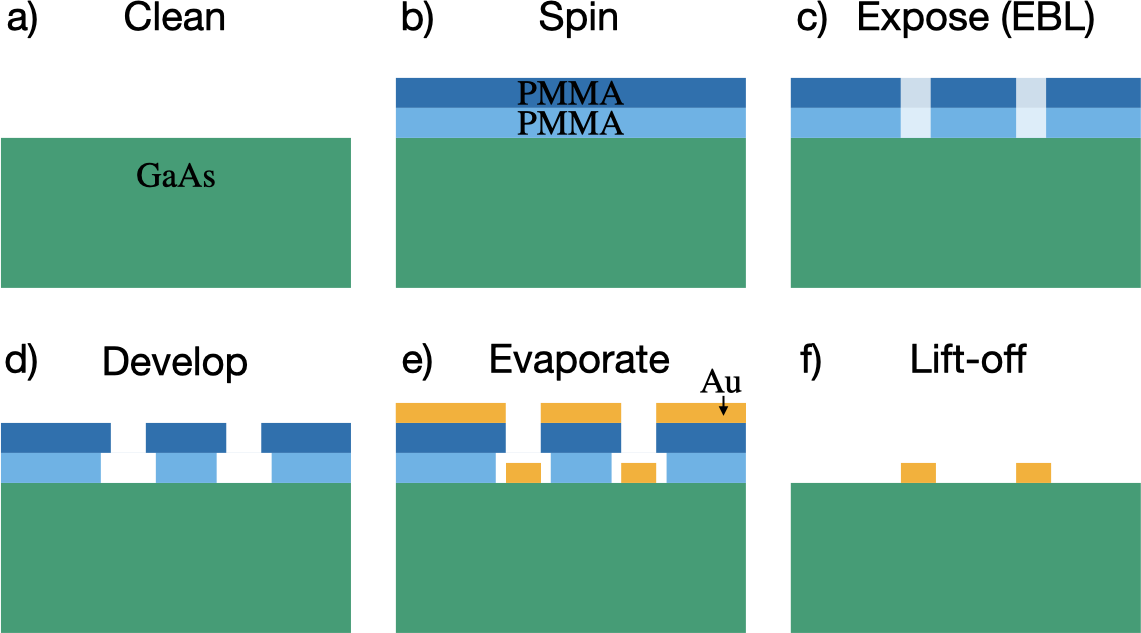
\includegraphics[width=1.0\textwidth]{figures/appendix/crop_FiguresMaster.020.png}
    \caption[Step-by-step diagram for fabricating metal gates]{\label{fig:appx/gate_fab} 
    (\textbf{a}) GaAs/AlGaAs heterostructure is cleaned in an Ultra-Sonic (US) bath with acetone/IPA/DI. 
    (\textbf{b}) Two different layers of PMMA are spun ontop of the heterostructure.
    (\textbf{c}) The gate design is exposed to an electron beam to breakup the PMMA.
    (\textbf{d}) The chip is developed in an IPA:DI solution create an undercut and remove the exposed PMMA.
    (\textbf{e}) 2:\qty{12}{nm} of Ti:Au are evaporated ontop of the chip.
    (\textbf{f}) The chip is rinsed in acetone to remove remaining PMMA and any metal attached to it. The chip is ready to be placed onto a chip carrier, wirebonded and measured.}
  \end{center}
\end{figure}